% Relatório do laboratório 5 de servo
% Felipe Bandeira da Silva
% 27/09/2013

%\documentclass[a4paper, 10pt]{article}
\documentclass[paper=a4, fontsize=11pt]{article}


\usepackage[brazil]{babel}
\usepackage[utf8]{inputenc}
\usepackage{listings}
\usepackage{color}
\usepackage{amsthm}
\usepackage{graphicx}

\usepackage{schemabloc}
\usetikzlibrary{circuits}

\setlength{\parindent}{0pt}
\setlength{\parskip}{18pt}

\title{Laboratório Transformadores\\O Autotransformador}
\author{Felipe Bandeira da Silva}
\date{}

\begin{document}


\maketitle

Este laboratório tem como objetivo: Estudar a relação de tensão e corrente de um autotransformador. 
Aprender como se liga um transformador para que trabalhe como autotransformador.

\newpage

\listoffigures

\newpage

\section{Fundamentação Teórica}

Até o momento em todas as experiências feitas no laboratório, foram utilizando o conceito
de isolamento entre primário e secundário. Propondo com isso uma isolação elétrica. Agora 
esse tipo de utilização apresenta um pequeno empecilho, as perdas por efeito Joule, Correntes
de Magnetização são intensificadas com o isolamento. Para que se possa aumentar o rendimento
de um transformador é utilizado uma configuração tal, que o enrolamento do primário é 
compartilhado com o secundário. Configuração esta conhecida como, autotransformador, que 
caracteriza o transformador. O cuidado com essa configuração é a perda da isolação, fato
este que deve ser estudado com cuidado e dependerá obviamente da aplicação. Teoricamente
um \textbf{autotransformador} é definido como um transformador que só tem um enrolamento. 
Um transformador com múltiplos enrolamento pode ser considerado um autotransformador, se todos os 
enrolamentos forem compartilhados, ou seja, ligados em série. Em adição ou oposição. Para
forma assim um único enrolamento. O esquemático clássico para o autotransformador  abaixador
é mostrado na Figura~\ref{abaixador},

\begin{figure}[!ht]
    \centering
    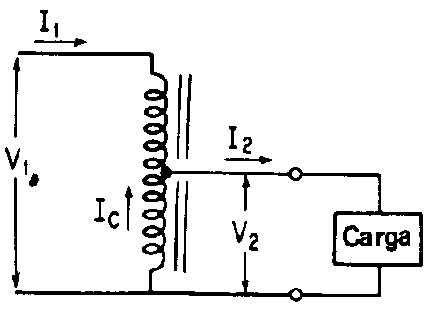
\includegraphics[scale=.4]{abaixador.png}
    \caption{Transformador Abaixador}
    \label{abaixador}
\end{figure}

Para a configuração elevador a única alteração é que o enrolamento com menor volta é
usado como primário, como segue na Figura~\ref{elevador},

\begin{figure}[!ht]
    \centering
    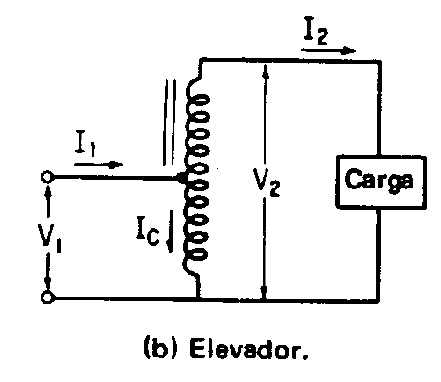
\includegraphics[scale=.4]{elevador.png}
    \caption{Transformador Elevador}
    \label{elevador}
\end{figure}

Um analise no sentido da corrente na configuração da Figura~\ref{abaixador}, mostra
que o sentido da corrente no secundário difere do que poderia ser esperado isso deve 
ao fato que o autotransformador deve obedecer a seguinte regra:

\begin{equation}
    V_1 I_1 = V_2 I_2
    \label{eq:v1i1}
\end{equation}

Portanto se $V_2$ é menor que $V_1$, $I_2$ deve exceder $I_1$. Assim para o circuito
mostrador na Figura~\ref{abaixador} a relação de correntes fica,

\begin{equation}
    I_2 = I_1 + I_c
\end{equation}

A Figura~\ref{elevador}, fecha a analise, de que, um autotransformador elevador, não
pode ser um divisor de tensão. Novamente, partindo da equação~\ref{eq:v1i1}, e 
$V_2 > V_1$, então $I_1 >  I_2$. Assim, para o circuito mostrado na Figura~\ref{elevador},

\begin{equation}
    I_1 = I_2 + I_c
\end{equation}

O autotransformador pode também ser feito variável, entretanto, da mesma maneira
que o potenciómetro é um divisor de tensão ajustável. 
\textbf{Autotransformadores variáveis} consistem num simples enrolamento, praticado
num núcleo de ferro toroidal, como é mostrado na Figura~\ref{variac}. Esta configuração
de construção dada para um autotransformador é caracteriza um autotransformador, 
conhecido como \textbf{variac}, onde uma escova de carvão pressa no eixo rotativo, que 
faz contato com as espiras expostas do enrolamento do transformador. Apesar da
construção mostrada na Figura~\ref{variac} ser usada como abaixadora, a simples
mudança da tensão de entrada ser no secundário, faz o Variac se tornar elevador.
Deve-se observar que a corrente instantânea na parte comum do autotransformador
$I_c$ pode circular em qualquer sentido, para cima ou para baixo, dependendo se
o transformador for usado como abaixador ou elevador. Assim, a única maneira
de determinar-se o sentido da corrente no enrolamento comum é analisando
as direções do primário e secundário, onde a diferença de  $I_c$ deve ser suprida.


\begin{figure}[!ht]
    \centering
    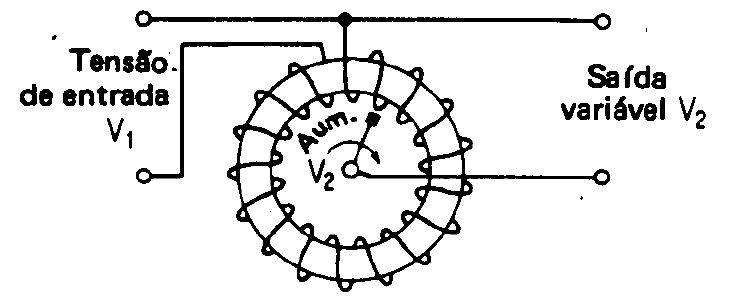
\includegraphics[scale=.4]{toroidal.png}
    \caption{Variac}
    \label{variac}
\end{figure}

Qualquer transformador comum, de dois enrolamento isolador, pode ser convertido
num autotransformador como mostra a Figura~\ref{isolador}.

\begin{figure}[!ht]
    \centering
    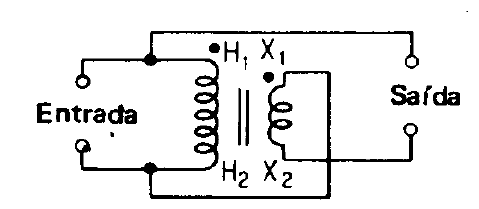
\includegraphics[scale=.4]{isolado.png}
    \caption{Transformador isolado para autotransformador, configuração aditiva}
    \label{isolador}
\end{figure}

Para a configuração aditiva o resultado, é exemplificado na Figura~\ref{isolador2},

\begin{figure}[!ht]
    \centering
    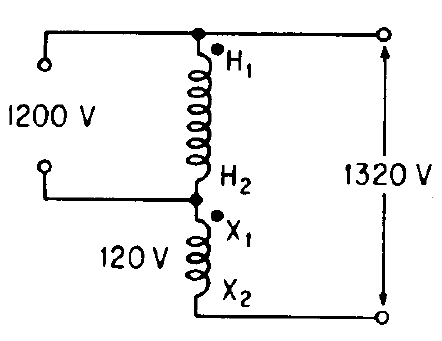
\includegraphics[scale=.4]{isolado2.png}
    \caption{Autotrasnformador configuração aditiva}
    \label{isolador2}
\end{figure}

Finalizando aqui a introdução teórica para uma configuração bastante utilizada na
industria.

\section{Experiência, Configuração Abaixador}

Para a experiência seguir será utilizado a configuração mostrada na 
Figura~\ref{abaixador}. Para tanto, foi monitorado as tensões de entrada e saída
respectivamente no primário e secundário do transformador. Foram feitas medições
na corrente de primário e secundário. Conectado uma carga puramente resistiva
no secundário, com valor de $120 \Omega$. Após a alimentação do
autotransforma com $120 V$. Os seguintes valores foram anotados,

\begin{center}
    \begin{tabular}{c||c||c}
        Medição & Valor & Unidade \\
        \hline
        $I_1$ & 0.25 & A \\
        $I_2$ & 0.475 & A \\
        $V_2$ & 58.7 & V \\
    \end{tabular}
\end{center}

A corrente de circulação $I_c$ é dada por $I_2 - I_1$ ficando portanto com 
valor de $225 mA$

A potências calculadas para os circuitos primário($S_{pri}$) e secundário($S_{sec}$) foram, 


\begin{center}
    \begin{tabular}{c||c||c}
        Potência & Valor & Unidade \\
        \hline
        $S_{pri}$ & 30 & VA \\
        $S_{sec}$ & 27.84 & VA \\
    \end{tabular}
\end{center}

O único cometário interessante a ser feito é a desigualdade numérica apresentada no 
item acima, teoricamente a potência consumida no primário deve ser igual a potência
do secundário. A única explicação plausível é que o transformador usado apresenta
perdas na transformação, perdas estas já conhecidas, efeito Joule, Resistência dos
enrolamento... Portanto os valores de potência são válidos para a pratica propostas
e podem sim serem considerados iguais. Concluindo com isso que o transformador
não é ideal. Mas funcional.

\section{Experiência, Configuração Elevador}

A experiência segue o esquemático mostrado na Figura~\ref{elevador}, onde a tensão
agora do primário não deve exceder $60 V$, respeitando a tensão nominal dos 
enrolamentos usados do modulo. Conectado agora uma impedância puramente
resistiva com valor de $600 \Omega$. Foram anotações os seguintes valores,

\begin{center}
    \begin{tabular}{c||c||c}
        Medição & Valor & Unidade \\
        \hline
        $I_1$ & 0.4 & A \\
        $I_2$ & 0.184 & A \\
        $V_2$ & 117.6 & V \\
    \end{tabular}
\end{center}

A corrente de circulação $I_c$ é dada por $I_1 - I_2$ ficando portanto com 
valor de $216 mA$.

A potências calculadas para os circuitos primário($S_{pri}$) e secundário($S_{sec}$) foram, 


\begin{center}
    \begin{tabular}{c||c||c}
        Potência & Valor & Unidade \\
        \hline
        $S_{pri}$ & 24 & VA \\
        $S_{sec}$ & 21.64 & VA \\
    \end{tabular}
\end{center}

Novamente se percebe uma diferença numérica para o transformador real, algo 
válido.

\subsection{Retirando a corrente de circulação}

A mudança proposta é que o terminal 6 do módulo seja desconectado fazendo com isso
um puro indutor, com os terminais da cargas curto-circuitados é possível facilmente
que a corrente no secundário será a mesma no primário. A corrente anotada para
o primário foi $I_1 = 49 mA$.


\section{Conclusão}

Esta experiência introduz ao estudante de engenharia Elétrica uma configuração
útil na regulação de linhas de transmissão, o autotransformador pode ser usado
em diversas situação, podemos aproveitar de seu alto rendimento com os devidos
cuidados com a falta de isolação, isolação está interessante para sistemas de potência.




\end{document}

